\chapter{Il progetto}

Il sito web di \MonIQA{} contiene diverse pagine, ognuna delle quali svolge una
funzione precisa: è presente una pagina che illustra l'algoritmo di calcolo
dell'indice IQA; una dove si possono reperire informazioni sui principali
inquinanti atmosferici; una mappa di tutte le stazioni di monitoraggio dislocate
sul territorio nazionale con calcolo degli indici e grafico dell'andamento
giornaliero per ogni stazione; un'altra per visualizzare informazioni aggregate
per regione; una pagina di ricerca che permette di visualizzare i dati di una
singola stazione per un singolo giorno; e infine una heat-map della
concentrazione delle stazioni di monitoraggio su tutto il suolo nazionale.

L'obiettivo di questo lavoro è stato quello di estendere \MonIQA{} aggiungendo
una nuova pagina, chiamata \controlname{Dati Storici}, che mostri, per area
geografica, informazioni aggregate sull'andamento (\textit{trend}) dell'IQA e
degli inquinanti nell'aria per ogni stagione in un determinato periodo
temporale.

Da un punto di vista dell'utente la pagina deve funzionare come segue:
\begin{enumerate}
	\item l'utente seleziona l'area geografica di interesse da una lista di
		tutte le aree geografiche disponibili;
	\item l'utente seleziona il range di anni in cui vuole esaminare
		l'andamento della qualità dell'aria;
	\item il sito mostra, in forma tabulare e con un grafico a linee, i
		valori dell'IQA e degli inquinanti per ogni stagione di ogni
		anno.
\end{enumerate}

La nuova pagina deve avere l'obiettivo di permettere di analizzare il trend
dell'indice di qualità dell'aria e degli inquinanti negli anni passati allo
scopo di fornire alle amministrazioni territoriali uno strumento utile ad
individuare i principali aspetti di interesse per combattere l'inquinamento e a
verificare, tramite l'analisi dei trend, se le scelte e gli investimenti
adottati hanno ottenuto i risultati previsti o meno.

Inoltre questo nuovo strumento deve permettere ai cittadini di potersi informare
sull'andamento della qualità dell'aria nella loro zona in modo che possano
efficacemente valutare l'operato delle amministrazioni locali nella lotta
all'inquinamento ambientale.

A tal fine, la pagina deve soddisfare alcuni requisiti fondamentali, di seguito
elencati.
\begin{itemize}
	\item Deve essere \emph{semplice e intuitivo}: lo strumento deve poter
		essere utilizzato anche da utenti non esperti.
	\item Deve avere un'\emph{interfaccia grafica pulita e ordinata}: è
		indispensabile che l'utente possa ricavare le informazioni di
		cui necessita dai dati mostrati nella pagina in modo immediato.
	\item Deve avere un \emph{grafico a linee} con l'andamento degli
		inquinanti nel tempo: fondamentale per poter facilmente
		visualizzare i trend.
	\item Deve mostrare le informazioni in modo da poter \emph{comparare i
		valori di inquinamento dell'aria di ogni anno con gli anni
		precedenti e successivi} negli stessi periodi di tempo.
	\item Deve permettere di \emph{filtrare i risultati} anche per singole
		stazioni (utile per analizzare lo stato dell'aria in zone di
		particolare interesse, come vicino a una zona industriale, a
		un'autostrada o a una scuola) e per singolo inquinante (per
		poter studiare l'andamento dell'inquinante nel tempo più in
		dettaglio).
	\item Deve disporre di una \emph{funzionalità che consenta all'utente di
		valutare l'attendibilità} dei dati mostrati.
\end{itemize}

Nei capitoli seguenti sono illustrate le soluzioni adottate per soddisfare i
requisiti sopra elencati oltre che per risolvere altri problemi sorti durante lo
sviluppo del software.

\section{Aree geografiche}\label{sec:areas}

La prima questione che si pone per la realizzazione del progetto, riguarda come
definire le aree geografiche che l'utente può selezionare come area da
analizzare. Trovare una soluzione a questo problema si rende necessario in
quanto, talvolta, nel database di \MonIQA{}, per alcune stazioni di
monitoraggio, sono presenti periodi di tempo in cui non sono disponibili
misurazioni.  Pertanto, si può limitare il problema aggregando insieme più
stazioni di monitoraggio. I dati aggregati così raccolti avranno minor
possibilità di contenere periodi privi di dati (risulta infatti improbabile che
mettendo insieme le informazioni provenienti da più stazioni ci siano intervalli
di tempo dove nessuna stazione ha raccolto dati). Le cause di questi vuoti di
dati possono essere varie: alcune stazioni di monitoraggio possono andare
\textit{offline} per alcuni periodi, oppure gli script che si occupano di
prelevare le misurazioni e inserirle nel database di \MonIQA{} possono smettere
di funzionare, e altro ancora.

Altro motivo per cui è importante definire aree geografiche è che l'obiettivo
del progetto è \emph{consentire l'analisi storica della qualità dell'aria di una
zona più o meno vasta}, e non solo di un singolo punto \idest{stazione di
monitoraggio}.

Pertanto, le aree geografiche da definire dovranno rispettare i seguenti
requisiti.
\begin{itemize}
	\item Devono essere \emph{sufficientemente vaste} da evitare troppi
		periodi privi di misurazioni nei dati aggregati.
	\item \emph{Non devono essere troppo vaste} per evitare di aggregare
		dati da stazioni di monitoraggio troppo distanti che,
		altrimenti, fornirebbero misurazioni di zone differenti del
		territorio nazionale, perdendo la validità di tali informazioni.
	\item Devono complessivamente \emph{coprire l'intero territorio
		nazionale}.
	\item Devono avere un \emph{nome chiaro che identifichi la zona} che si
		vuole analizzare. L'utente, infatti, dovrà poter selezionare
		l'area di suo interesse a partire dal nome.
\end{itemize}

Per rispondere a tali requisiti si è deciso di utilizzare \emph{le province e le
città metropolitane} (che chiameremo indifferentemente ``province'' nel
seguito).  Infatti, questi enti territoriali, non sono né eccessivamente vasti
né troppo piccoli e hanno tutti il nome di una città capoluogo che identifica
chiaramente l'area geografica. Inoltre, dato che il servizio ha anche
l'obiettivo di essere utile alle amministrazioni territoriali per valutare piani
e investimenti da attuare per ridurre l'inquinamento, una suddivisione basata
sui territori di competenza delle amministrazioni provinciali risulta
ragionevole.

Nel database di \MonIQA{} per ogni stazione di monitoraggio è presente un campo
\idest{colonna} ``città'' che relaziona la stazione con la città in cui si trova
(una descrizione dettagliata del database è fornita nel paragrafo successivo).
Nel database, gran parte dei record contengono il valore \code{NULL} in questo
campo, in quanto non tutte le stazioni si possono chiaramente assegnare a una
città (alcune stazioni si trovano in zone periferiche). Pertanto, al fine di
rimuovere questi valori \code{NULL} così da avere ogni stazione con una città
associata, si è deciso di utilizzare questo stesso campo della tabella delle
stazioni per associarle alle province: quindi ogni stazione non avrà più una
città di appartenenza, ma una provincia.

Nel database sono presenti quasi \(1000\) stazioni di monitoraggio, sarebbe
quindi scomodo assegnarle manualmente una per una alla relativa provincia.
Pertanto si è deciso di utilizzare uno script scritto in linguaggio Python
(\code{fill-cities.py}) che:
\begin{enumerate}
	\item preleva dal database la latitudine e la longitudine di ogni
		stazione di monitoraggio;
	\item utilizza un servizio esterno\footnote{Si è deciso di utilizzare il
		servizio \textsc{MapIt} fornito dall'Associazione Openpolis
		all'indirizzo \url{http://mapit.openpolis.it}.  Tale piattaforma
		fornisce una REST API che permette di ottenere, in formato JSON,
		informazioni sulle aree amministrative che circondano un punto
		geografico fornito tramite parametri di una richiesta HTTP
		GET\@. \textsc{MapIt} utilizza i dati sui confini delle unità
		amministrative rilasciati pubblicamente ogni anno dall'ISTAT.}
		per determinare la provincia in cui si trova la stazione di
		monitoraggio;
	\item produce uno script SQL che contiene le istruzioni \code{INSERT}
		che aggiungono le province nell'apposita tabella del database e
		le istruzioni \code{UPDATE} che aggiornano il campo ``città''
		delle stazioni in modo da associarlo alla provincia a cui
		appartengono.
\end{enumerate}

Si è deciso di generare uno script SQL piuttosto che modificare direttamente il
database, così da consentire all'utilizzatore dello script Python di revisionare
il risultato prima di eseguirlo sul server.

Lo script Python stampa le istruzioni SQL su stream \textit{standard output},
mentre sullo stream \textit{standard error} fornisce informazioni su quanto lo
script sta facendo (la stazione che sta processando e la provincia individuata)
e su eventuali errori.  In tal modo, è possibile utilizzare le funzioni di
redirezione dell'output fornite dal sistema operativo per produrre lo script SQL
su file senza rinunciare a controllare l'andamento dell'esecuzione.

\section{Prelievo dei dati dal database}\label{sec:database}

Il database di \MonIQA{} è strutturato, per la parte che interessa per questo
progetto, come nel diagramma in Figura \vref{fig:dbarch}.

\begin{figure}[htb]
	\centering
	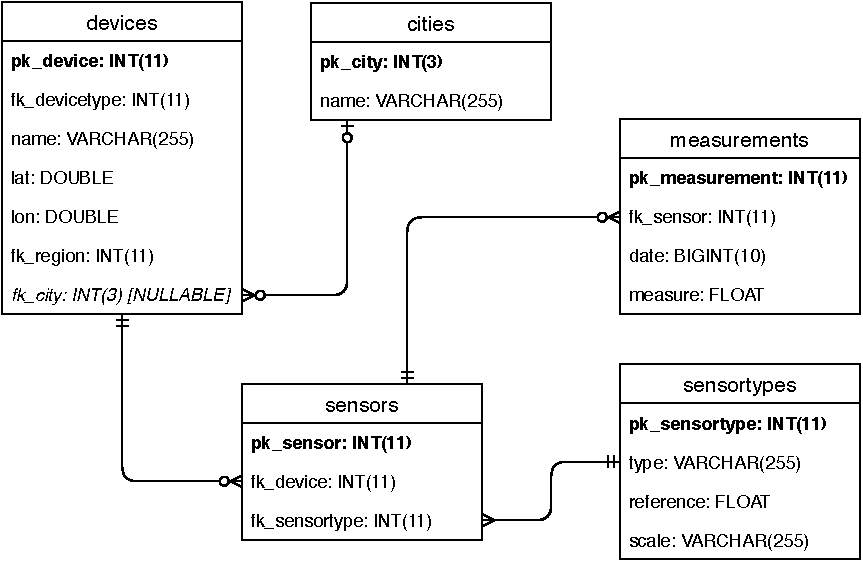
\includegraphics[width=\textwidth]{img/dbarch}
	\caption{Diagramma E-R del database di \MonIQA\@.}\label{fig:dbarch}
\end{figure}

La tabella \code{devices} contiene le stazioni di monitoraggio. Il campo
\code{fk\_city} è quello utilizzato per associare una provincia a ogni stazione,
come descritto nel paragrafo precedente. La tabella \code{cities} contiene
quindi le province.

La tabella \code{sensortypes} contiene un record per ogni tipo di sensore che
può essere installato sulle stazioni (i sensori si differenziano in base
all'inquinante che possono misurare) con il nome dell'inquinante che misurano, i
valori legali di riferimento e l'unità di misura per l'inquinante.

La tabella \code{measurements} contiene le misurazioni provenienti dai sensori
installate sulle stazioni, con il valore misurato e la data della misurazione.

Infine la tabella \code{sensors} mette in relazione le tabelle \code{devices},
\code{measurements} e \code{sensortypes} così da poter associare a ogni
misurazione la stazione e il sensore che l'ha effettuata.

Quindi, per prelevare i dati dal database, è stata sviluppata la query riportata
nel Listato \vref{lst:slowquery}.

\lstinputlisting[language=SQL, label={lst:slowquery}, caption={Query per il
prelievo dei dati dal database.}]{slow-query.sql}

In \code{\{\{PROVINCE\_NAME\}\}} andremo ad inserire il \emph{nome della
provincia} della quale si vogliono prelevare i dati; in
\code{\{\{START\_YEAR\}\}} e \code{\{\{END\_YEAR\}\}} inseriremo invece \emph{il
primo e l'ultimo anno del periodo di interesse}.

Divisioni e moltiplicazioni per \(1000\) sono necessarie in quanto, nel
database, tutte le date sono salvate come il numero di \emph{millisecondi}
trascorsi dalla mezzanotte del 01/01/1970, mentre le funzioni di MySQL
richiedono il numero di \emph{secondi} trascorsi da tale data.

La query ritorna quindi record aggregati per ogni anno, per ogni quarto di anno
e per ogni tipo di sensore \idest{inquinante}, fornendo la \emph{media delle
misurazioni di quel periodo per quell'inquinante} e \emph{il numero totale di
misurazioni} su cui la media è stata calcolata.

\section{Performance della query}

La query presentata nel paragrafo precedente ha però il difetto di avere
performance scarse. Ad esempio, eseguendo la query per la provincia di XXX
vediamo che impiega Y minuti per fornire il risultato. Tempo ovviamente non
accettabile per un'applicazione web.

Per ridurre il tempo richiesto per l'esecuzione della query si è quindi deciso
di aggiungere una nuova tabella al database che contiene già i dati aggregati
necessari e si aggiorna, attraverso \textit{trigger} MySQL, ogni volta che viene
aggiunta, modificata, eliminata una misurazione.

La nuova tabella, chiamata \code{historical\_data}, è definita come mostrato nel
Listato \vref{lst:historicaldatatable}.

\lstinputlisting[language=SQL, label={lst:historicaldatatable}, caption={Schema
della tabella \code{historical\_data} e dell'istruzione \code{INSERT} utilizzata
per riempire la tabella con tutte le misurazioni già presenti nel
database.}]{historical-data-table.sql}

I campi \code{year}, \code{quarter} e \code{fk\_sensortype} contengono,
rispettivamente, l'anno, il quarto di anno e la chiave esterna al tipo di
sensore. Il campo \code{fk\_city} contiene la chiave esterna alla provincia. I
campi \code{measure\_sum} e \code{measure\_count} contengono invece la somma di
tutte le misurazioni (per quella provincia, quarto di anno e tipo di sensore) e
il numero totale di misurazioni disponibili.  La media può essere calcolata come
\(measure\_sum / measure\_count\). In questo modo abbiamo realizzato una tabella
che fa da ``cache'' per i dati aggregati che vogliamo ottenere e possiamo
utilizzare la query mostrata nel Listato \vref{lst:fastquery} per prelevare i
dati.

\lstinputlisting[language=SQL, label={lst:fastquery}, caption={Query ottimizzata
per il prelievo dei dati dal database.}]{fast-query.sql}

Le performance sono molto migliorate. Infatti la nuova query, sempre per la
provincia XXX, ritorna il risultato in soli Z secondi.

Tre trigger MySQL si occupano di mantenere aggiornata tale tabella ad ogni
operazione di \code{INSERT}, \code{UPDATE}, \code{DELETE} sulla tabella
\code{measurements}. L'aggiornamento non richiede alcuna operazione
\textit{resource-intensive} in quanto, ad esempio, per l'inserimento di una nuova
misurazione, è sufficiente individuare il record da aggiornare (in base al
periodo, alla provincia e al tipo di sensore della nuova misurazione), quindi
sommare a \code{measure\_sum} il valore della nuova misurazione e incrementare
di uno il contatore \code{measure\_count}.

\section[User-experience e visualizzazione dei dati]{User-experience e
visualizzazione\\dei dati}

Per fornire all'utente un'interfaccia grafica semplice e intuitiva si è deciso
di utilizzare gli eventi JavaScript per accompagnare l'utente in una procedura
guidata per l'inserimento dei parametri di ricerca. Tutto il codice JavaScript
(dove, per comodità, si fa uso anche della libreria jQuery) è stato inserito nel
file \code{dati-storici.js}.

In particolare, la pagina mostra inizialmente una \textit{drop-down list} dove
l'utente può selezionare la provincia di suo interesse tra tutte quelle di cui
sono disponibili dei dati. Una volta selezionata la provincia, il codice
JavaScript effettua una richiesta POST in tecnologia AJAX a
\code{getYearRange.php}, che esegue una query SQL sul database e ritorna, in
formato JSON, il range massimo di anni per cui sono disponibili misurazioni per
la provincia selezionata \idest{il primo e l'ultimo anno presenti nella tabella
\code{historical\_data}}. Questo range è utilizzato dal JavaScript per riempire
un'altra drop-down list --- quella dove l'utente può selezionare l'anno iniziale
per il periodo di interesse, che viene mostrata solo dopo che la richiesta POST
si è conclusa (inizialmente nascosta) --- con tutti gli anni compresi nel range
(estremi inclusi). In tal modo, possiamo garantire che l'utente non possa
scegliere range di anni troppo grandi che conterrebbero anni senza misurazioni e
complicherebbero inutilmente la visualizzazione dei dati.

Quindi, quando l'utente seleziona l'anno iniziale del periodo di suo interesse,
l'applicazione mostra una terza drop-down list nascosta per selezionare l'anno
di fine. Dopo che l'utente ha selezionato anche l'anno di fine, il codice
JavaScript invia una richiesta AJAX POST a \code{getHistoricalData.php} che
preleva i dati richiesti dalla tabella \code{historical\_data} e li ritorna in
formato JSON.

Infine, attraverso un'altra richiesta AJAX POST, questa volta a
\code{getDevicesByCity.php}, viene prelevata la lista di tutte le stazioni di
monitoraggio presenti nella provincia selezionata e viene inserita in un'altra
drop-down list che consente di filtrare i dati per stazione. Viene quindi
mostrata anche l'ultima drop-down list che consente di filtrare i dati per
inquinante: in questa lista vengono inseriti solo gli inquinanti per i quali
sono disponibili dati per la provincia o stazione selezionata, in modo che
l'utente non possa selezionare inquinanti per i quali non sono presenti
misurazioni.

In Figura \ref{fig:ux} è possibile vedere un esempio di compilazione di tutte
le drop-down list da parte dell'utente.

\begin{figure}[htb]
	\centering
	
\includegraphics[width=\textwidth]{img/ux}
	\caption{Esempio di compilazione delle drop-down list che costituiscono
	l'interfaccia grafica della pagina.}\label{fig:ux}
\end{figure}

Per quanto riguarda la visualizzazione dei dati si è deciso di dividerla in due
parti: in una prima parte viene mostrata una tabella dove, per ogni anno e per
ogni quarto di anno, sono presentati: il maggior inquinante rilevato nell'aria,
relativamente al suo limite di riferimento; l'indice IQA percentuale calcolato
sul maggior inquinante (con relativo cromatismo mostrato con un piccolo cerchio
colorato); la variazione rispetto allo stesso quarto dell'anno precedente e di
due anni precedenti dell'IQA in termini percentuali (colorata di rosso se
positiva e di verde se negativa).

Sotto questa tabella viene anche mostrata la media percentuale dell'IQA per il
primo anno del range selezionato \idest{la media percentuale dell'IQA per i 4
quarti d'anno che compongono l'anno iniziale selezionato dall'utente} e per
l'ultimo anno del range. Quindi viene dato un giudizio globale (Migliorato,
Peggiorato o Invariato) basato sulla differenza tra queste due medie.

Qualora siano presenti dei buchi nei dati, questi dovranno comunque comparire in
tabella mostrando un trattino per indicare che per tale anno o periodo non sono
disponibili misurazioni. Questo permette di avere una tabella uniforme dove tra
una riga e l'altra c'è sempre la differenza di un solo quarto di anno.

La funzione che si occupa di generare il codice HTML per mostrare la tabella è
\code{getTableInnerHTML()}.

Un esempio di tabella, per la provincia di Milano per il periodo 2015--2019, è
mostrato in Figura \ref{fig:datatable}. Si noti come dalla tabella si può
facilmente dedurre che:
\begin{itemize}
	\item complessivamente, la qualità dell'aria è mediocre: l'IQA varia tra
		l'\(83\%\) e il \(176\%\), tenendosi il più delle volte sopra il
		\(100\%\);
	\item durante l'autunno e l'inverno (Q1 e Q4) l'inquinante maggiormente
		presente è il \(\chem{PM2.5}\) mentre durante la primavera e
		l'estate (Q2 e Q3) il più presente è l'\(\chem{O_3}\). Questo è
		in linea con quanto previsto, infatti le maggiori attività
		dell'industria e il più intenso traffico veicolari nelle città
		durante le stagioni fredde contribuiscono a far aumentare il
		particolato sottile nell'aria, mentre con il caldo e il maggior
		irraggiamento solare del periodo estivo si hanno le condizioni
		per attivare i processi chimico-fisici che portano alla
		formazione dell'ozono troposferico a partire dagli ossidi di
		azoto;
	\item nel corso degli anni, la qualità dell'aria a Milano è
		progressivamente migliorata: nei primi anni sono presenti molti
		cerchi rossi (qualità scadente) mentre non sono presenti negli
		ultimi due anni; inoltre le variazioni dell'IQA mostrano
		prevalentemente decrementi (verde) con pochi incrementi (rosso).
		La stessa informazione si può ricavare dal giudizio globale in
		fondo alla tabella.
\end{itemize}

\begin{figure}[htp]
	\centering
	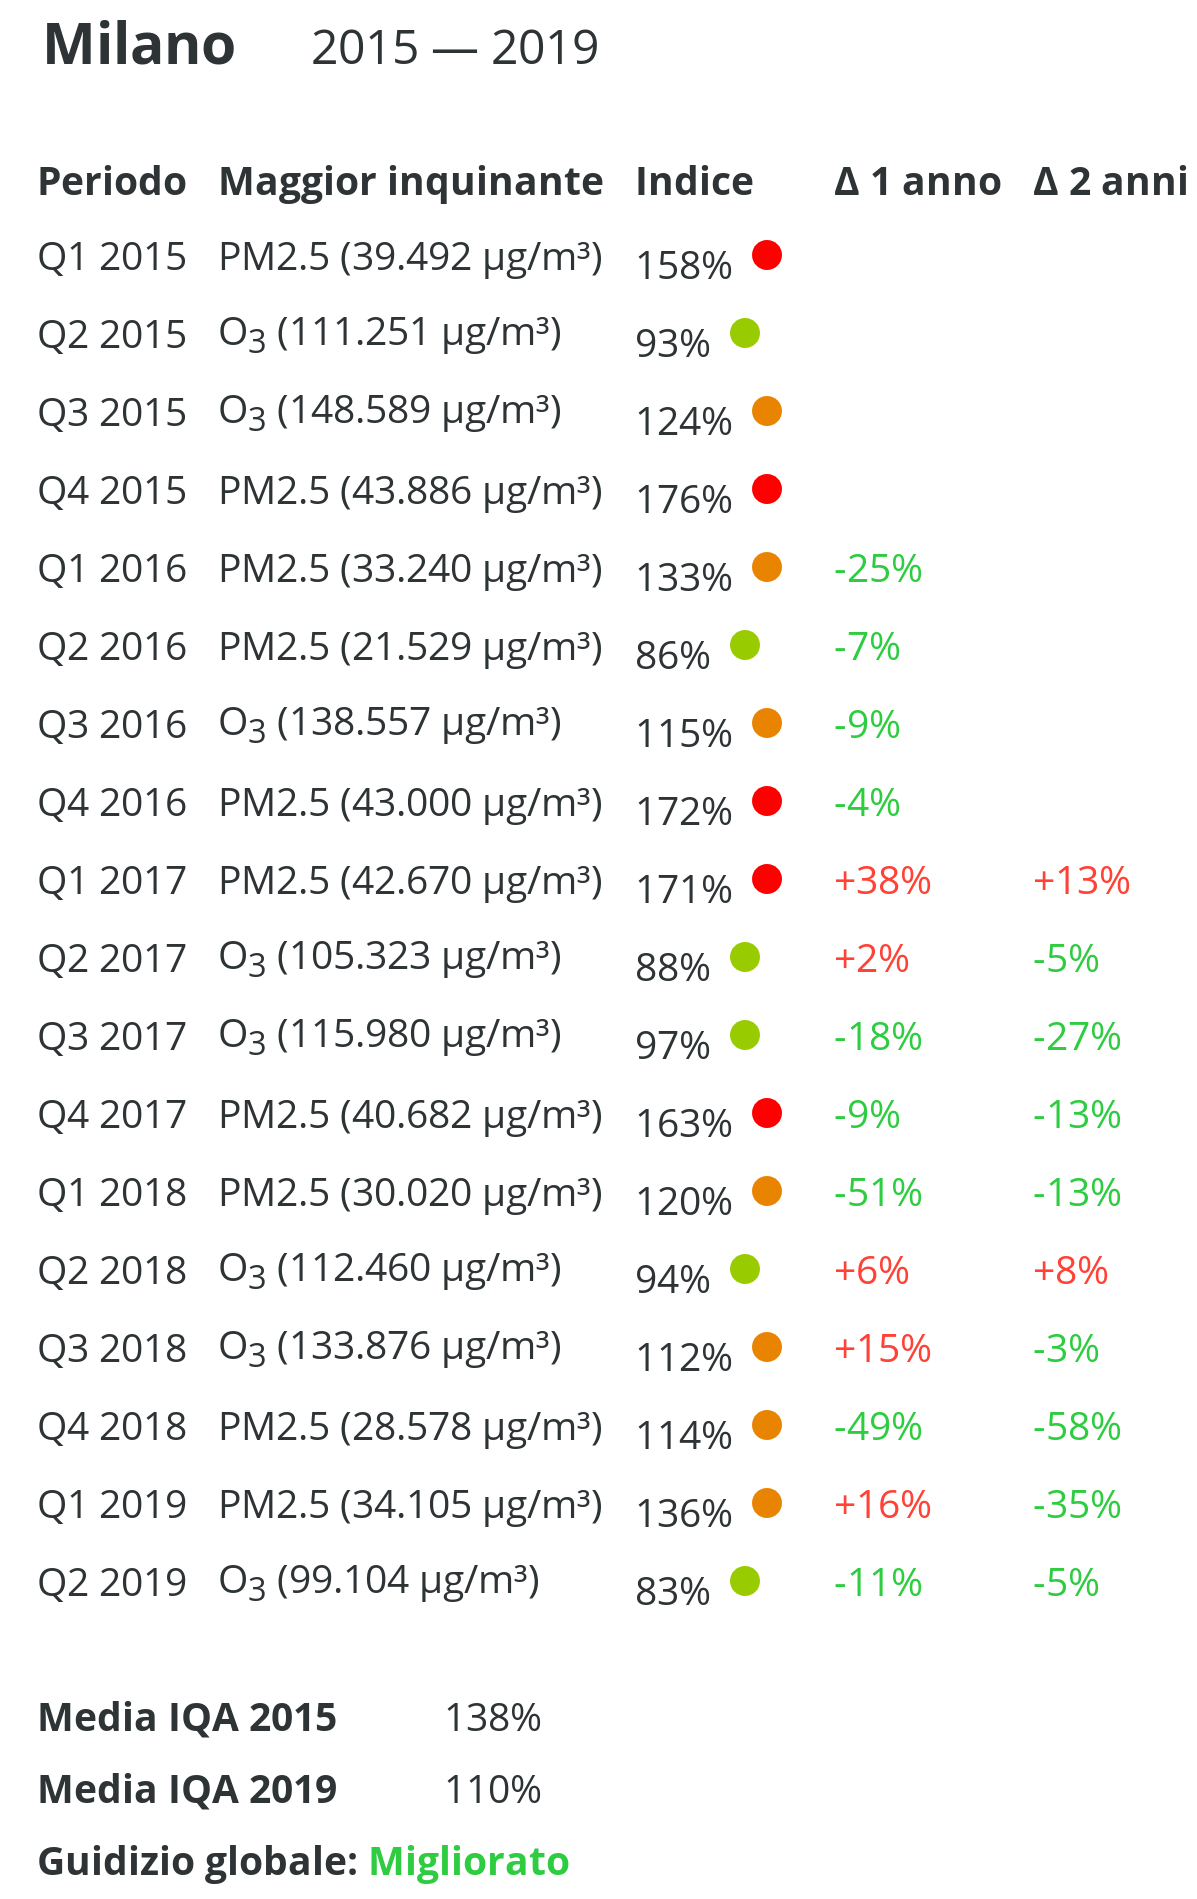
\includegraphics[width=0.7\textwidth]{img/datatable}
	\caption{Tabella della provincia di Milano per il periodo
	2015--2019.}\label{fig:datatable}
\end{figure}

Sotto alla tabella è mostrato anche un grafico dove viene illustrato l'andamento
di ogni inquinante (ogni linea corrisponde a un inquinante). Dal grafico,
realizzato con la libreria Google Charts, è possibile individuare immediatamente
trend e oscillazioni nella concentrazione degli inquinanti nell'aria.

La funzione che si occupa di inizializzare il grafico e inserire i dati è
chiamata \code{showGraphData()}.

In Figura \ref{fig:graph} è mostrato il grafico della provincia di Pisa per gli
anni 2014--2019. Si nota facilmente che:
\begin{itemize}
	\item l'ozono troposferico (\(\chem{O_3}\)) è in un trend leggermente
		rialzista, ed è maggiormente presente nei periodi caldi;
	\item il biossido di azoto (\(\chem{NO_2}\)) segue un trend ribassista,
		ed è maggiormente presente nei periodi freddi con l'incremento
		del traffico veicolare;
	\item la concentrazione degli altri inquinanti è generalmente rimasta
		invariata nel tempo e mostrano dei picchi durante il periodo
		invernale.
\end{itemize}

\begin{figure}[htp]
	\centering
	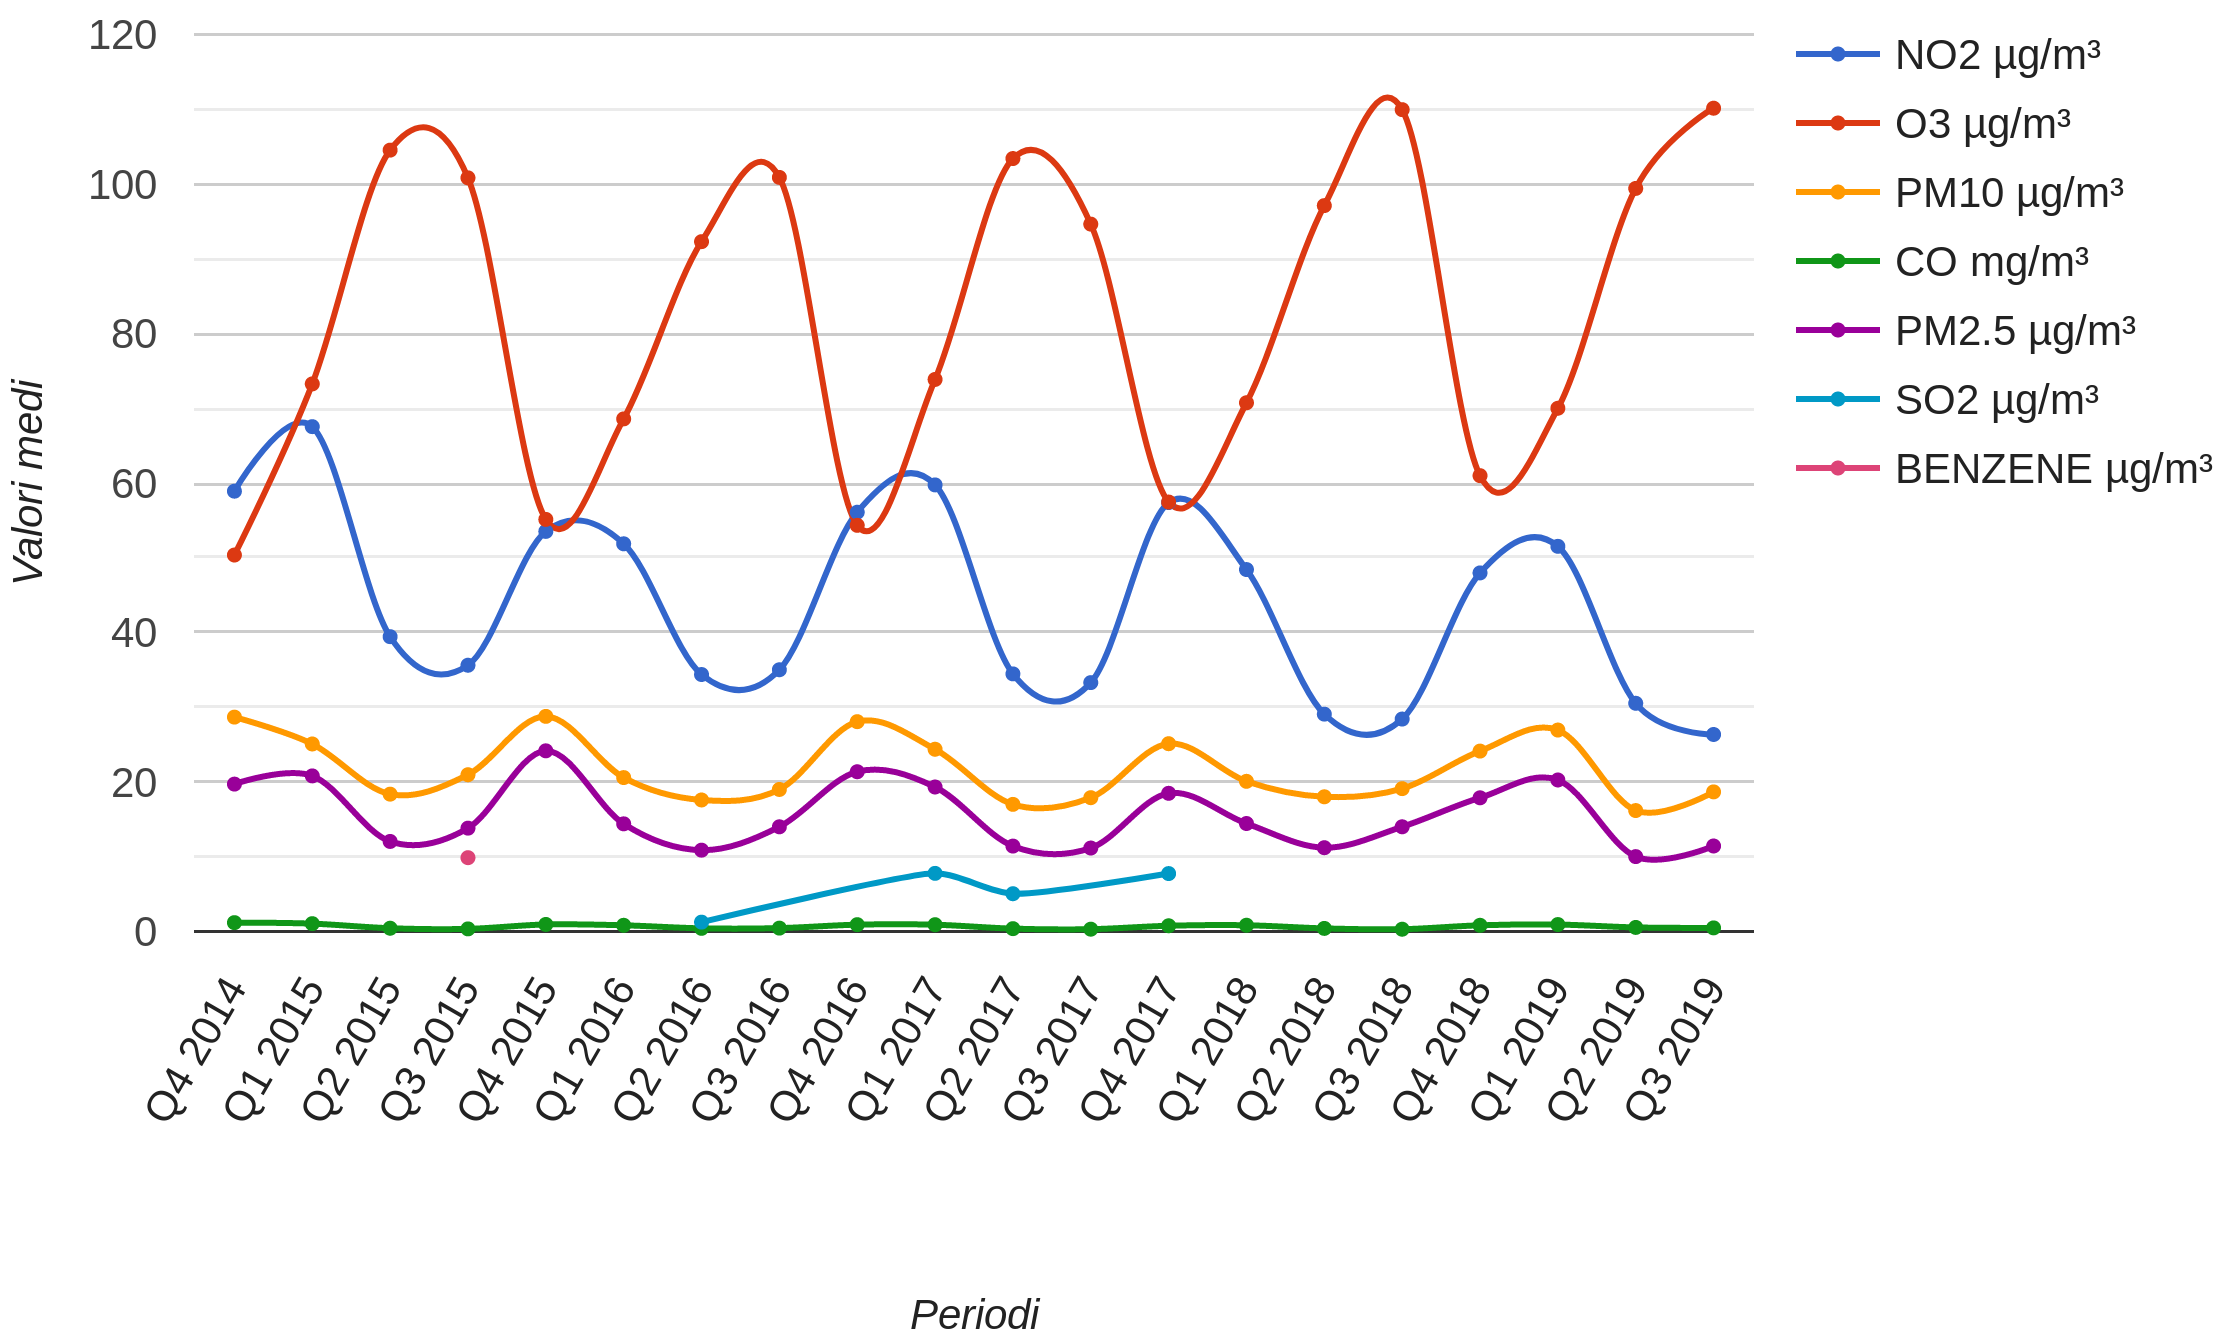
\includegraphics[width=\textwidth]{img/graph}
	\caption{Grafico per la provincia di Pisa per il periodo
	2014--2019.}\label{fig:graph}
\end{figure}

Portando il cursore su un qualsiasi punto delle linee del grafico, l'utente può
controllare il valore medio delle misurazioni dell'inquinante in quel punto e,
al fine di valutare l'attendibilità di tale valore medio, il \emph{numero totale
di misurazioni} su cui è stata svolta la media.

\section{Filtraggio dei dati}

Una volta ottenuti i dati, l'applicazione \textit{client-side} \idest{lo script
JavaScript \code{dati-storici.js}} può opzionalmente filtrarli per stazione o
per inquinante. Due drop-down list forniscono all'utente la lista di tutte le
stazioni presenti nella provincia selezionata e tutti gli inquinanti per i quali
sono disponibili misurazioni.

Per filtrare per inquinante, è sufficiente utilizzare solo i dati aggregati
relativi all'inquinante selezionato dall'utente per riempire i valori della
tabella e del grafico Google Charts. Di questo si occupa la funzione
\code{changingPollutantFilter()}.

Per filtrare invece per stazione non possiamo utilizzare i dati aggregati in
quanto non contengono le informazioni sulle stazioni che hanno effettuato le
misurazioni. Pertanto, quando l'utente seleziona una stazione dalla lista, è
necessaria una nuova richiesta AJAX POST al server che esegue la query seguente
per ottenere i dati per la sola stazione selezionata.

La query è eseguita dallo stesso script \code{getHistoricalData.php} che
discrimina le richieste di dati aggregati per provincia o per singola stazione
in base a quali parametri POST vengono utilizzati nella richiesta.

La query ha buone performance in questo caso, dato che deve prelevare i dati di
una singola stazione e non di tutte le stazioni di una provincia, quindi anche
il numero di misurazioni totali è molto ridotto.

In seguito al filtraggio (sia per stazione che per inquinante) il codice
JavaScript utilizza una struttura dati identica a quella utilizzata per i dati
non filtrati. Pertanto possiamo sfruttare il riutilizzo del codice per mostrare
i dati nella tabella e nel grafico.

In Figura \vref{fig:filtering} è mostrato un esempio di filtraggio sia per
stazione che per inquinante per la provincia di Pisa.

\begin{figure}[p]
	\centering
	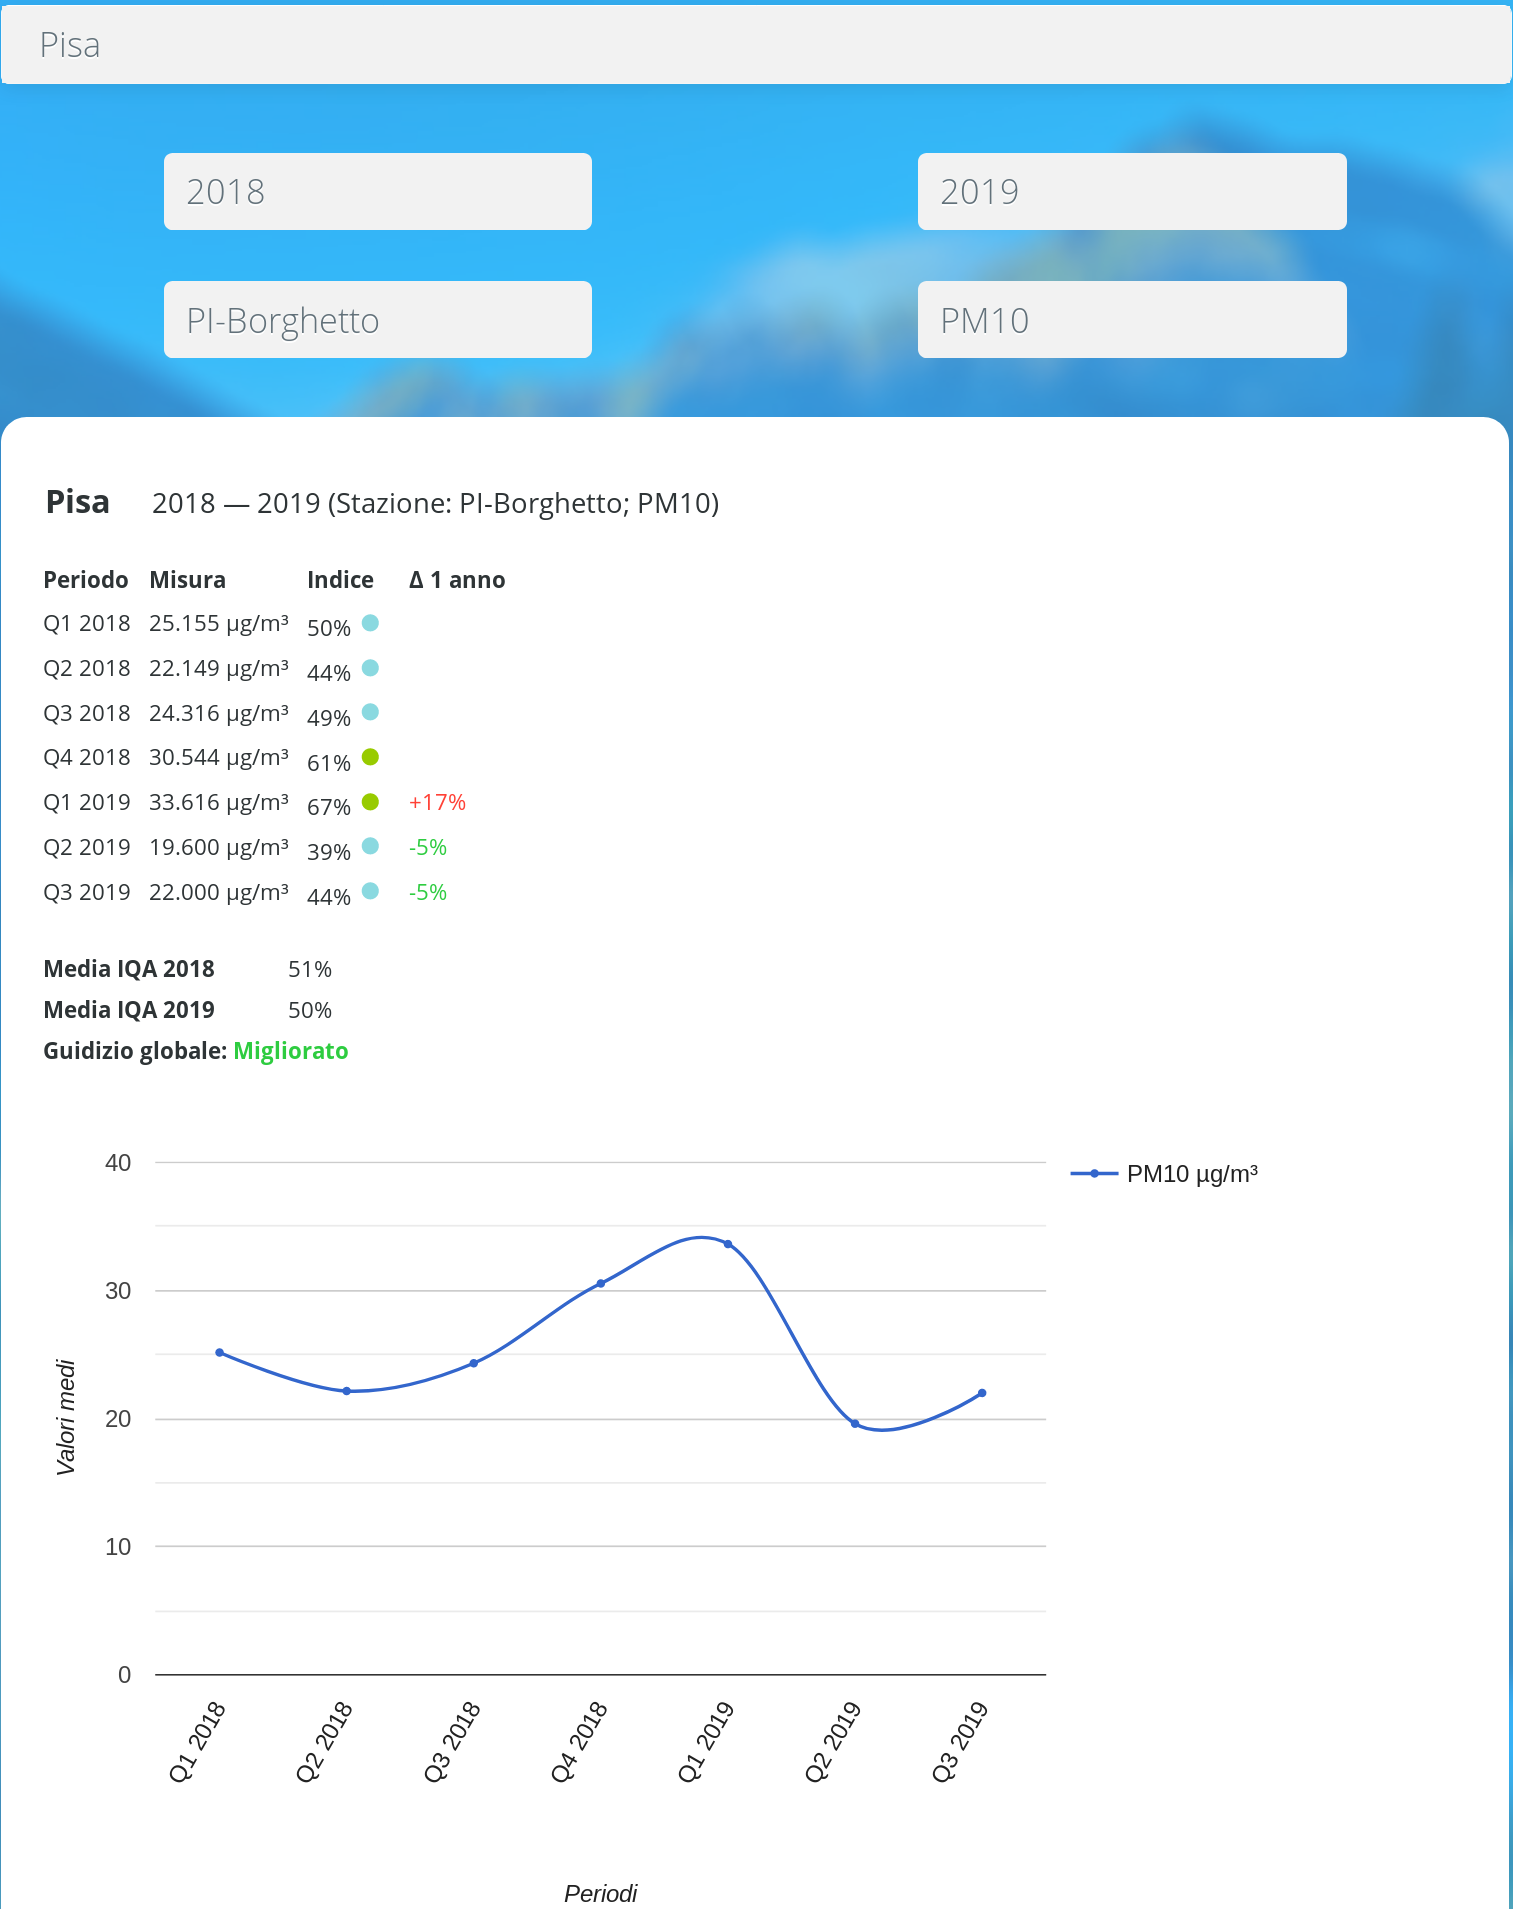
\includegraphics[width=\textwidth]{img/filtering}
	\caption{Esempio di filtraggio per stazione e per inquinante per la
	provincia di Pisa.}\label{fig:filtering}
\end{figure}

